\documentclass{article}
\usepackage[a4paper, total={6in, 8in}]{geometry}
\usepackage[backend=bibtex]{biblatex}
\addbibresource{bibfileold.bib}
\usepackage{array}
\usepackage{caption}
\usepackage{subcaption}
\usepackage{authblk}
\usepackage[pdfborder={0 0 0}]{hyperref}% For email addresses
\usepackage{titlesec}
\titleformat{\section}
  {\normalfont\fontsize{12}{15}\bfseries}{\thesection}{1em}{}



\title{Climate change in the Andes: a case of agent-based modeling for anticipatory policy making}

\author[1]{\normalsize Jos\'{e} Manuel Magallanes}
\author[2]{\normalsize Claudio Cioffi-Revilla}
\affil[1,2]{\small  Center for Social Complexity\\
George Mason University \\
\url{{jmagalla,ccioffi}@gmu.edu}}
\affil[1]{\small eScience Institute and Evans School of Public Policy\\
University of Washington\\
\url{magajm@uw.edu}}
\affil[1]{\small Department of Social Sciences\\
Pontificia Universidad Catolica del Peru\\
\url{jmagallanes@pucp.edu.pe}}


\usepackage{Sweave}
\begin{document}
\Sconcordance{concordance:MagallanesCioffiPaper.tex:MagallanesCioffiPaper.Rnw:%
1 30 1 1 0 1 1 1 4 419 1}


\maketitle

\begin{abstract}
Can climate change alter habitats so that emigration and social conflict can happen in a place currently consider peaceful and as a good destination to immmigrate? How can all the current and dispersed knowledge be combined so that political decision makers be better informed? This works informs of such a case where climate change is modifying different variables that may trigger conditions difficult to foresee with a linear approach. Particularly, we used an agent-based model to capture the complexity of the coupling of the natural and social systems in Huancayo, a city in the central Andes of Peru, and it is shown how the current conditions can give rise to the emergence of social conflict and emigration from this location, currently living in peace and representing one of the most attractive regions to live in.

\end{abstract}


\section{Introduction}

This work has collected information related to the current trends on water balance, population growth, and glacier melting in the most important city of the central Andes of Peru, Huancayo. As these trends may continue, we want to know what are the potential social issues that may arise, namely:
\begin{itemize}
\item Is it possible that drastic migration patterns appear?
\item Is it possible the emergence of social conflict in the area?
\end{itemize}

This work supports the hypothesis that those questions have affirmative answers, if no anticipative action is carried on timely. To test this hypothesis, we have organized multiple sources of knowledge and information into  a logical account of this possibility. From there, we have built an agent-based model to transform this knowledge into an interdisciplinary computational tool. This will allow us to foresee different scenarios that may arise from our logical assumptions and information available. 

The area chosen, Huancayo\footnote{We are using the name of the Province of Huancayo, but we are precisely dealing with the area that comprises the political Districts of Huancayo, El Tambo and Chilca that depend on the water from the Shullcas River.}, is currently under study by different scholars and institutions whose objectives are similar yet lacking inter disciplinary integration. Different public  research institutes are working to produce either glaciological, hydrological or climatological updates on the area; isolated researchers are doing small-scale models to whether alert of different local water risks or propose adaptation programs in the communities more likely to be affected by the nature trends; while political authorities agenda is dominated by a modernization discourse that sees in the growth of cities the unavoidable sign of progress. This situation has led to a partition of the problem of water scarcity in the area and its implications among national, regional and local public officers and politicians, where each tries to solve a piece. So as of today, no model exists to allow  knowledge integration and support political coordination. 

Water scarcity and droughts have an slow onset, so as time passes by, the majority of urban and rural settlers do not pay much attention to this issue. These people in the watershed are not experiencing a critical condition, or at least not worse than the country-wide average conditions. In this situation, this work is presented in the right moment to serve as an input for  anticipative political decisions, as neither are effective measures currently implemented. However, the presence of different actors with different goals and beliefs, makes it challenging for mainstream modeling techniques to provide the right guidance, so this work hopes to contribute methodologically to avoid a negative future for Huancayo.

\section{Literature Review}

Research interests dealing with climate change are varied, but they tend to have a common interest in rural populations, especially vulnerable and located in developing countries. Ziervogel et al.\cite{ziervogel_agent-based_2005} focuses on modeling decision-making and forecasting of farmers in Lesotho, in an scenario where official forecasts, besides poorly done, are not diligently nor appropriately disseminated towards these end-users, making them more vulnerable as loses due to poor information endanger the farmers\textquotesingle survivability. The same research design is also found in Bharwani et al. \cite{bharwani_multiagent_2005} for smallholder farmers in a village in Vhembe district, Limpopo Province, South Africa. More recent and more comprehensive approaches are found in Kniveton et al. \cite{kniveton_agent-based_2011} and Hailegiorgis \cite{hailegiorgis_computational_2013}. The former has Burkina Fasso as its case study, investigating the role of the environment in the decision to migrate using scenarios of future demographic, economic, social, political, and climate change in a dry land context. In that work, these authors found that change to a drier environment produces the largest total and international migration fluxes when combined with changes to inclusive and connected social and political governance, while the lowest international migration flows are produced under a wetter climate with exclusive and diverse governance scenarios. And the latter focuses on the South Omo zone in southern Ethiopia, modeling how the current surge in large-scale land acquisition might affect rural livelihood. In his work,  Hailegiorgis found that (i) the occurrence of drought affects their adaptive capacity and forces migration; (ii) increasing the magnitude of expansion of large-scale land acquisition aggravate dispossession and increase migration of rural households; and (iii) capacity building and relief support in the time of extreme events minimizes migration. All of these techniques make use of agent-based models using diverse platforms (Netlogo \cite{wilensky_introduction_2015}, Mason \cite{luke_mason_2015}, and AnyLogic \cite{anylogic_2015}).
\par
As it is clear so far, climate change stresses the place where human activities are carried out, thus deteriorating the quality of the environment of these populations forcing them to make different decisions, which, as Hirschmann proposes \cite{hirschman_exit_1970}, can be categorized as exit, voice and loyalty. The previous cases speak of exit, as people emigrate looking for better conditions as the climate threatens their well-being; but, the confrontational and loyalty dimensions in social complexity issues also need to be analyzed under climate change effects. However, loyalty and voice seem to be less treated from the global computational social science community, which should be considered quite shocking as reports related to climate change and conflicts are abundant \cite{hendrix_climate_2012,hsiang_quantifying_2013,steinbruner_climate_2013}. Related to conflict and climate change, Piontek \cite{piontek_impact_2010} studies the Nile River, which serves 10 countries in Africa, seeking to understand, via computational modeling, how the interaction between humans and the environment may lead to conflict or cooperation. In this work, the author found that climate change can alter conditions for conflict and cooperation, but is very unlikely it is the immediate cause for those issues. Nevertheless, the most outstanding work related to climate change and the emergence of conflicts can be found in the works produced at the Center for Social Complexity at George Mason University the projects funded by the Multidisciplinary University Reserach Initiative (MURI) and Cyber-Enabled Discovery and Innovation (CDI) programs \cite{cioffi-revilla_methodology_2010,hailegiorgis_agent_2010,kennedy_agent-based_2010}. The former focuses on the complex interaction of pastoral groups with their environment and other emerging external actors in east Africa finding that increased seasonal rainfall variability and droughts create tremendous stress on pastoralists groups and challenges their long-term resilience and adaptive response mechanisms, thus concluding the population\textquotesingle s relation to the carrying capacity seems to be the major factor affecting cooperation and conflict. The latter, still unfinished, focuses on how human communities in Africa and the northern hemisphere respond to changing climate.  


My research complements the current studies in many directions: 
\begin{itemize}
\item First, the object of study is not a particular kind of population (as it is the case in most studies) but it studies simultaneously vulnerable but not marginal rural populations, and an urban population of the close metropolitan area; so the water issues will be of concern to two different kind of groups with different necessities on water, which may be the starting point for inter group conflict \cite{bar-tal_intergroup_2011}. 
\item Second, this agent based model will include the effect of a glacier in the water supply for the social system, facilitating the analysis of similar systems by separating the precipitation (rainfall and snowmelt). 
\item Third, the watershed under analysis may be a representative case for the whole Andes chain, as it is at the center, among the dry biggest cities on the west and the sparsely inhabited Amazon jungle to the east. 
\item Fourth, it will integrate and harmonize current modeling efforts on the glacier melting trend, the hydrology dynamics and the social behavior; making our work more challenging as these systems have never been integrated before bringing into question the validity of our results. 
\item Finally, and related to the previous point, the issue is not of particular concern neither to the majority of the population nor to the political authorities; it looks as though nobody wants to touch the situation as it may collide with the current way people live and benefit. This work also continued with the best practices in computational social science (CSS) research used by the previous studies, as it  integrated the complex adaptive systems approach \cite{miller_complex_2007}, the CSS consolidated techniques \cite{cioffi-revilla_introduction_2014}, and ethnographic work \cite{crate_anthropology_2009}.
\end{itemize}

\section{Overview and building blocks}

This work has the general goal of producing a base case interdisciplinary model to represent \emph{a possible} future for Huancayo as the water balance becomes insufficient to satisfy the population\textquotesingle s needs. We consider this model as a coupled human-natural system, where the model keeps the current trends in both systems and sees whether it is possible to see emigration and social conflict emerge.

The product of this work is an agent-based model programmed in Netlogo \cite{wilensky_introduction_2015}, which will follow a complex adaptive systems approach, when needed. The model respects particular characteristics of complex adaptive systems: there are many agents interacting dynamically, the agents have bounded rationality, i.e., only aware of local information, the agents have ways to establish networks which helps them get information, and history matters as path dependence emerges from the agent decisions. However, this complexity is well \emph{encapsulated} into the model, so the non-expert user can interact with it and even contribute to its improvement. 

As the social and natural systems have huge amounts of components, this agent-based model needs to abstract carefully the more important components to capture the  relationships hypothesized while still be useful for policy making. Thus, the social system will basically represent the demographics of the area and the urbanization growth; and the natural system will represent the water balance built form the glacier melting and rainfall trends. This is represented in Figure \ref{scheme}, we have two interacting subsystems. For each subsystem, we have collected different kinds of data.

\begin{figure}[ht]
  \centering
  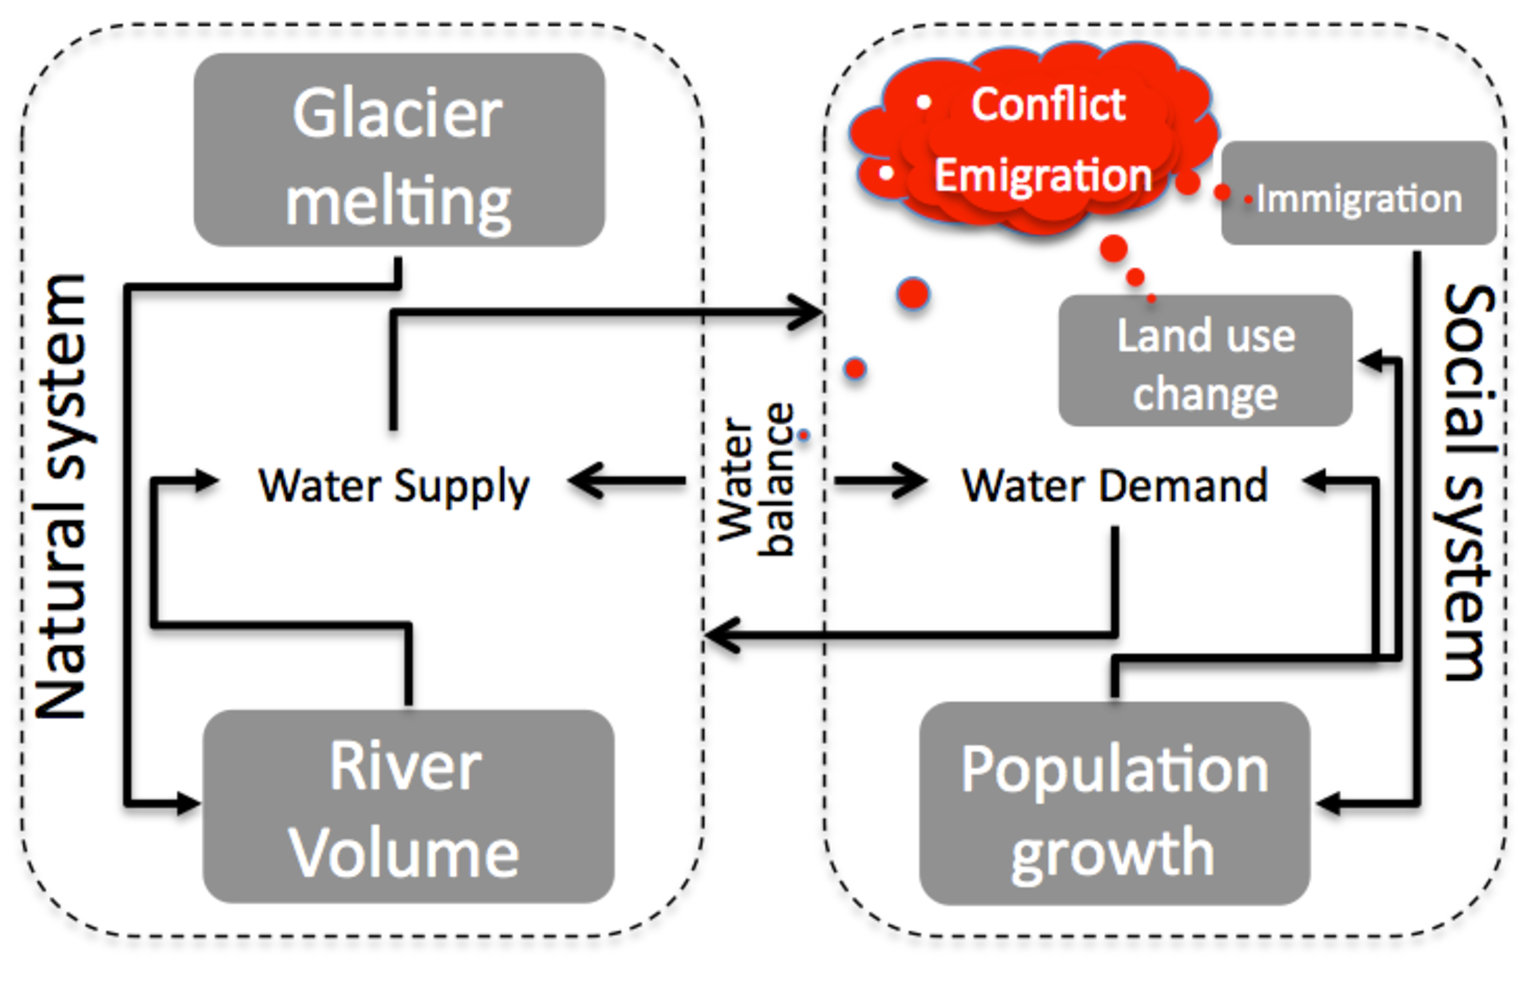
\includegraphics[width=0.5\textwidth]{modelsummaryGraph}
  \caption[Basic model abstraction]{Basic model abstraction. The red elements represent the potential outcomes if the other elements keep the current trends}
  \label{scheme}
\end{figure}

In the natural system, this work focuses on the water supply, as it is the key trigger factor for the social issues of interest in this work. Due to that importance, much emphasis has been placed in collecting data to feed the model with a credible water balance model. As water balance depends on the supply and demand of water, the natural system is responsible for the water supply, which depends mainly on rainfall and snow melting. As the official reports on water supply consider these dimensions only, we have not dared to include more components. The current trend in the natural system proposes both a decreasing supply of rainfall and forecasts the complete retreat of the glacier, which will affect the balance negatively \cite{carlos_riesgos_2012,lopez-moreno_recent_2014}. One obstacle for a more precise model is the lack of information on the snow melt supply, but we will manage to bound that value by eliciting expert opinions and recent measurements available. 

On the other hand, water demand comes from the social system, which is represented by two subsystems, rural and urban. The basic process in both sub systems is population growth, that is, eventually there will be not enough water supply for the population\textquotesingle s demand. We explore emigration as a particular response (other responses have not been considered at all): there are not many Andean cities having positive population growth but Huancayo metropolis is one of them, so making a case for the opposite phenomenon is politically important. Following the field work on this area, this model tries to give the agent options to avoid migration as water scarcity increases, but the limited local space and agent\textquotesingle s satisfaction will eventually leave him no more option than migrate. Another set of demographic variables for the agents are their working, educational and marital status, which are used in the moment the urban agent decide \emph{where} to migrate, that is, those values constrain their free will to chose between moving to the coast or the jungle. We have also considered the immigration parameters in this area, considering that currently Huancayo hosts immigrants from poorer communities nearby, which will be a key factor for conflict to emerge. Precisely speaking, we present a basic heuristic to represent a situation when rural agents are eager to go into conflict due to the present of \emph{strangers} in their neighborhood during extreme water scarcity. As it is clear, conflict is a process that can emerge from the urban and rural area, while migration emerges from the urban area, and not from the rural area, following the results of our field work. However, for a rural agent to migrate, it first needs to have moved to the urban area; and for an urban agent to be perceived as a stranger by a rural one, it needs to have immigrated from another place and established its home in the neighborhood of a rural settler suffering water stress.

\section{Hypothesis Operationalization}

As this work proposes that the research questions have affirmative answers, we propose the following operationalization of variables in the hypothesis, as described in Figure \ref{operational}:

\begin{figure}[h]
%%%\figSpace
  \centering
  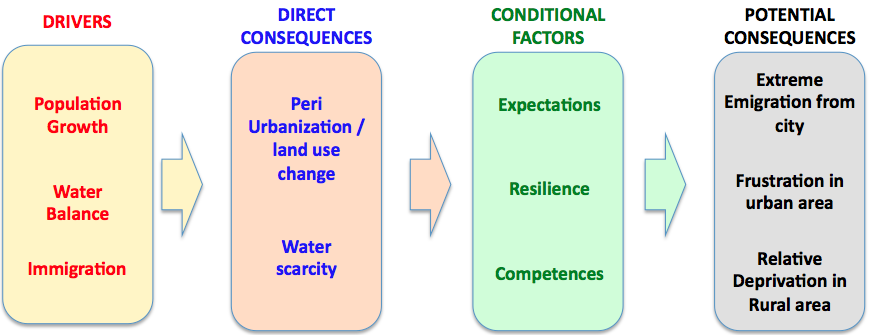
\includegraphics{operational}
  \caption[Operational Variables in Hypothesis]{Operational Variables in Hypothesis}
  \label{operational}
  %%%\figSpace % This adds separation
\end{figure}

The variables present a simple yet comprehensive process to study the potential for conflict and migration:
\begin{itemize}
\item The {\bf potential outcomes} are chosen as the representation of our framework \emph{exit, voice and loyalty}\cite{hirschman_exit_1970}. In this case, \emph{exit} is represented by {\bf drastic migration}; \emph{loyalty} by the permanence in Huancayo (not shown); and \emph{voice} by expected reaction from the {\bf frustration} felt urban people, or the {\bf relative deprivation} felt by rural people . 

\item The {\bf drivers} clearly represent the current trends in Huancayo  in the social and natural dimensions. This work proposes a model where these trends are not altered and will show how other factors included explicitly in the model could be managed to prevent the potential outcomes. The assumption that the trends can be extended into the future are based on the historical growth of Huancayo, an example of lack of urban planing since its creation. The social trends are population growth and immigration into Huancayo. Population growth already includes the migration balance, but the parameters of immigration into Huancayo will be used explicitly in the model, as the non Huanca presence is important for the the direct and potential consequences of the model. The water balance trend represents the other important driver, which will be represented by water supply and demand. Water supply will particularly pay attention to the contribution of the glacier Huayatapallana to the hydrology of the system. 

\item The {\bf direct consequences} are the clear results of the unaltered trends. Based on the dynamics of Huancayo , we have chosen the two most clear direct consequences supported by the literature and field work \cite{haller_huancayo_2013,ho_2012,haller_vivid_2012}. Water scarcity is a first expected outcome as the water balance and population growth trends remain unaltered. Water scarcity will become a major problem (as explained in \cite{carlos_riesgos_2012} and detailed in the next chapter) in the near future, which will combine with population growth and, particularly, immigration to exacerbate peri urbanization and land use change \cite{haller_huancayo_2013,haller_vivid_2012,ho_2012}. 

\item The {\bf conditionant factors} are processes that work at the individual level, and are the main sources of hetereogeneity in the model. Every individual will need to find an particular response based on these factors. The factors have been selected from the classical work of Maslow \cite{maslow_motivation_1987} (see Figure \ref{maslow}) and its application in agent based modeling to understand conflictive situations \cite{watkins_understanding_2008}. According to this individual level factors, we implemented a Bayesian mechanism to compute expectations, we carried out field work to uncover the local resilience, and made use of the census data to derive the competences of each individual. The competences reflect closely what determines the potential outcomes \cite{watkins_understanding_2008}, that is, of water (physiological needs), work (safety needs), family (belonging needs) and education (for steem and self-realization needs).  

  \begin{figure}[h]
  %%%\figSpace
    \centering
    \includegraphics[width=0.65\textwidth]{maslow}
    \caption[Hierarchy of Maslow]{Pyramid showing Maslow's hierarchy of needs.}
    Source: From \url{http://psychclassics.yorku.ca/Maslow/motivation.htm}
    \label{maslow}
    %%%\figSpace % This adds separation
  \end{figure}

\end{itemize}



\section{Field work}

We decided to organize an ad-hoc collection of information in situ as the model required some information for the agents not available in the literature. We needed to have a clearer idea on how the agents will react as water will become scarce in the rural and urban area. For that reason, We organized two research expeditions for each area.

\subsection{Research on rural area}

The rural area represents the longest extension of land in this work, but is also the less populated. People inhabitting the rural are very sensible to the variations of water balance. However, these people are also well trained to survive in these conditions.  As our model has an hypothetical scenario of water scarcity, the team had to be very careful to present this scenario to the people they interviewed. 

The goal of this expedition was to uncover:
\begin{enumerate}
\item \emph{Are urban people aware there might be water issues in the future?}
\item \emph{How long a rural person can stand water scarcity before migrating?}
\item \emph{What would it take for a rural person suffering water scarcity to feel relatively deprived?}
\end {enumerate}


The rural team lived in the rural area. They established their center of operations at Acopalca, in a shelter used for tourists. From there, the team visited the herders (higher altitudes) and the farmers (lower altitudes). Each time they visited a family, a team member informed that they were studying how climate change could impact their environment and ask for permission to accompany them in their habitual activities. That is, the main strategy was \emph{participant observation}, a technique chosen to gain better familiarity with the rural people and uncover in a valid way the information needed for the field work goals. The main findings were very surprising. First, person after person affirmed that drastic migration is not an option for the rural. And second, the increasing presence of non Huanca urbanizing the rural area represented an unappealing fact. The study also confirmed people were very aware of the progressive diminishment of water, but are also aware that it has not affected them. For sure, they believe this issue will be of more concern in the urban area, not in theirs.

A couple of additional important facts were unveiled. First, they are sure that the urban needs of water will collide with the rural needs. They know water is enough for rural life, but are not sure how much water will the growing city may need in the future. They are not confident local authorities will consider their opinion if the city needs more water. Second, they believe this generation of rural people will do their best effort to make a living in the rural area; but they are not very sure what would be the reaction of the future generations. They consider that the jungle represent an attractive destination for young unemployed people, but are afraid the attaction comes from easy-money and illegal activities.

\subsection{Research on urban area}

The urban expedition started in January 2015. The team for this expedition was composed only by local anthropologists from the Universidad Nacional del Centro del Peru, in Huancayo. 

The peri urban expedition worked between January and March 2015. As the goal quote was 50 families, the team needed to oversample (15 extra households) as not every selected household cooperated. The team learned that a \emph{fake} marketing company had once made interviews in the area, but they were in fact thieves that used the information to steal cars in the neighborhood. This data colection followed a different approach. In this case, a survey was designed and applied to 50 families living in the urbanizations located in the limit between the city and the rural area. The team designed a polietapic sampling design to include a representative sample of households in the urban settlements located along the peri urban area (see Table \ref{urbansample}).



\begin{table}[ht]
%%\tableSpace % This adds separation
\centering
\caption{Composition of Urban sample for this study}
% latex table generated in R 3.0.2 by xtable 1.7-3 package
% Tue Jul 14 02:37:16 2015
\begin{tabular}{lr}
 Urban Settlement & Sample quote \\ 
  \hline
Chorrillos &   5 \\ 
  Santa Martha &   5 \\ 
  Corona del Fraile &   5 \\ 
  Centenario &   7 \\ 
  La Floresta II &   6 \\ 
  Las colinas de San Antonio &   5 \\ 
  La Merced &   7 \\ 
  El Remanso &   5 \\ 
  Torre Torre &   5 \\ 
   \hline
Total &  50 \\ 
  \end{tabular}\label{urbansample}
%%\tableSpace % This adds separation
\end{table}


The goal of this expedition was the similar to the previous one, but including more topics, considering that the urban area will be the one suffering more scarity. This is detailed in Table \ref{urbanq}:

\begin{table}[ht]
%%\tableSpace % This adds separation
\centering
\caption{Protocol followed by urban expedition}
{\scriptsize
% latex table generated in R 3.0.2 by xtable 1.7-3 package
% Tue Jul 14 02:37:16 2015
\begin{tabular}{m{2in}p{1in}p{1.7in}}
  \hline
Guiding questions & Question type & Typical answers obtained \\ 
  \hline
How long an urban person can stand water scarcity before migrating? & Value requested in years & [4,5,6] \\ 
  What would an urban person do when water scarcity is felt at home? & Open question & Look for place nearby or migrate \\ 
  What would it take for a urban person suffering water scarcity to feel frustrated? & Open question & Difficulty to migrate \\ 
  What is the origin of the peri urban settlers? & Boolean question & Huanca or Non Huanca \\ 
  How did they end up living in that peri urban area? & Open question & Looking for a cheaper place \\ 
   \hline
\end{tabular}
}
\label{urbanq}
%%\tableSpace % This adds separation
\end{table}

From the table above, we obtained key considerations for the implementation of the model. First, we confirmed urban people have migration among their alternatives in case of lack of water with a resilience between 4 and 6 years. This is different from the current position shared by rural settlers. This is perfectly understandable as people in the city and in the peri urban area are already suffering episodes of water shortage during the dry season. The shortages are during some hours and are informed in advanced by the water company (SEDAM Huancayo).  Second, if the urban settlers predict that there will be permanent scarcity in the place they live, they will look for a place in Huancayo to move in. They are aware that they may need to get land closer to the rural area. It is worth noticing that all who said they will never migrate are non Huancas as they already did their investment to come to Huancayo. Third,   Huancas or non Huancas  believe that they will feel frustrated if they have to stay in place with water scarcity. Huancas would prefer to migrate, but if they can not, they will feel frustrated. Non Huancas do not wish to migrate ever, but staying in scarcity conditions will make them feel frustrated too. Fourth, the team found that the current share of non Huancas in the peri urban area was 45\%. And finally, we found out that people in the peri urban area did not start living in that zone but renting a place downtown, which was expensive, smaller and overcrowded. Progressively, they moved (renting or buying) into the peri urban area as it represented a cheaper place to live. The strategy they followed to find a better place was a system of references, where family and friends were sharing their experience living outside the center, even with lack of public utilities in the begining. In case of searching for water, they say they will follow the same strategy (referencing system from relatives).

The field work allowed us to complement the quantitative data available with some basic decision making mechanisms the rural and urban agents will adopt in case of this potentil scenario. Besides, the information from the field work will help us introduce heterogeneity in the agents. We consider that within the limitations for this research we have enough information to produce an informative model that will bring sufficient information for policy makers to start anticipatory thinking in the problem this model presents.After the field work, the relevant areas considered for this work were covered (see Figure \ref{etno} on page \pageref{etno})]. 

\begin{figure}[h]
%%%\figSpace
  \centering
  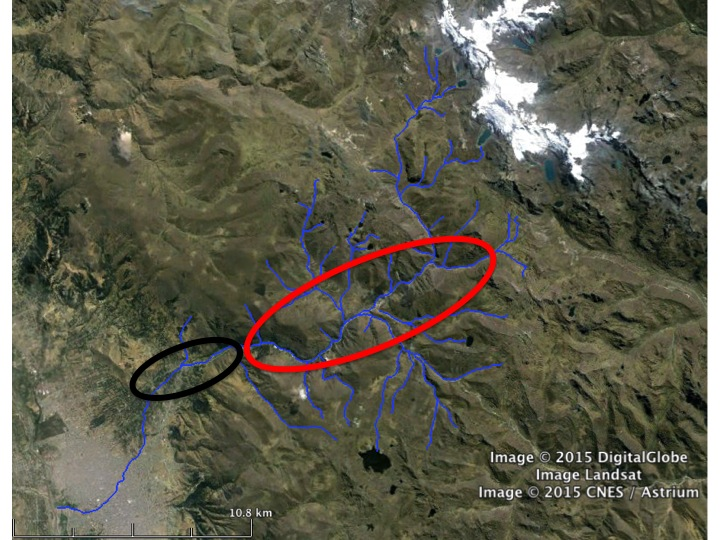
\includegraphics[width=0.6\linewidth]{etno}
  \caption[Map of Field work]{Map of Field work. The black oval is the area covered by the urban expedition and the red oval the area covered by the rural expedition}
  \label{etno}
  %%%%\figSpace % This adds separation
\end{figure}

\section{Modeling paradigm}

With all the data colected we had a good narrative to suppoirt our hypothesis. Nevertheless, even though narratives are needed for good modeling, they may not be good enough for making better decisions. Even if we added more details to our current narratives, those would be more details to the premises which increase the complexity of the narrative while maintaining or reducing the usefulness of our modelling efforts; as more assumptions will be needed the inferences will weaken, then this logical system will experience the Bonini\textquotesingle s Paradox \cite{bonini_simulation_1963}. This is when Computational Social Science comes into play in modern science, as Herbert Simon says:
\begin{quote}
\emph{``The obvious point is that, even when we have correct premises, it may be very difficult to discover what they imply. All correct reasoning is a grand system of tautologies, but only God can make direct use of that fact. The rest of us must painstakingly and fallibly tease out the consequences of our assumptions... Greatly oversimplified, the idea is that we already know the correct basic assumptions, ..., but we need the computer to work out the implications of the interactions of ... variables. ... For it is typical of many kinds of design problems that the inner system consists of components whose fundamental laws of behavior mechanical, electrical, or chemical are well known. The difficulty of the design problem often resides in predicting how an assemblage of such components will behave''}\cite{simon_sciences_1996}.
\end{quote}
Complexity is not a new concept, but the use of computers has allowed us to find better ways to understand emerging properties of complex systems \cite{simon_sciences_1996}. There are certainly many computational modeling approaches---e.g. system dynamics or discrete systems simulations---that deal with organizational complexity. However, key concepts such as learning and emergence can only be modeled, arguably, through the use of agent-based models (ABM) \cite{cioffi-revilla_introduction_2014,miller_complex_2007,gilbert_simulation_2005,epstein_growing_1996}. As with all modeling techniques, ABMs need to capture the most basic variables and processes that could explain a particular phenomenon, while making all building assumptions explicit and transparent, and producing outcomes valid and of interest to the scientific and policy community. In contrast to other techniques, agent-based models are virtual laboratories that allow their components to have different behaviors, reactions, and to be aware of only limited information. In particular, ABMs are useful in the social sciences when a particular social theory can be enacted through coding. We all can then see how the model behaves as the building parameters of the theory are manipulated \cite{miller_complex_2007,epstein_growing_1996}. Besides, ABM allows for the inclusion of complementary theories and models to carefully enrich the original theory, allowing the creation of different scenarios.


With this in mind, we created AndesLab. AndesLab starts in 2011, and simulates the next 50 years of Huancayo. Every time a complete cycle of the simulation is run, the history of Huancayo advances six months.  So, this model will only run for 100 cycles. As each cycle represents six months, a cycle represents a season, which is either the \emph{dry season} (that goes from May to September) or the \emph{rainy season} (that goes from October to April); so, the reasoning does not follow the January - December calendar. Figure \ref{flow1} reflects the flow of the code each cycle or season, a figure that also represents the translation of the concepts represented in the scheme \ref{scheme} on page \pageref{scheme} into computer logic. 

\begin{figure}[ht]
%%\figSpace
\centering
  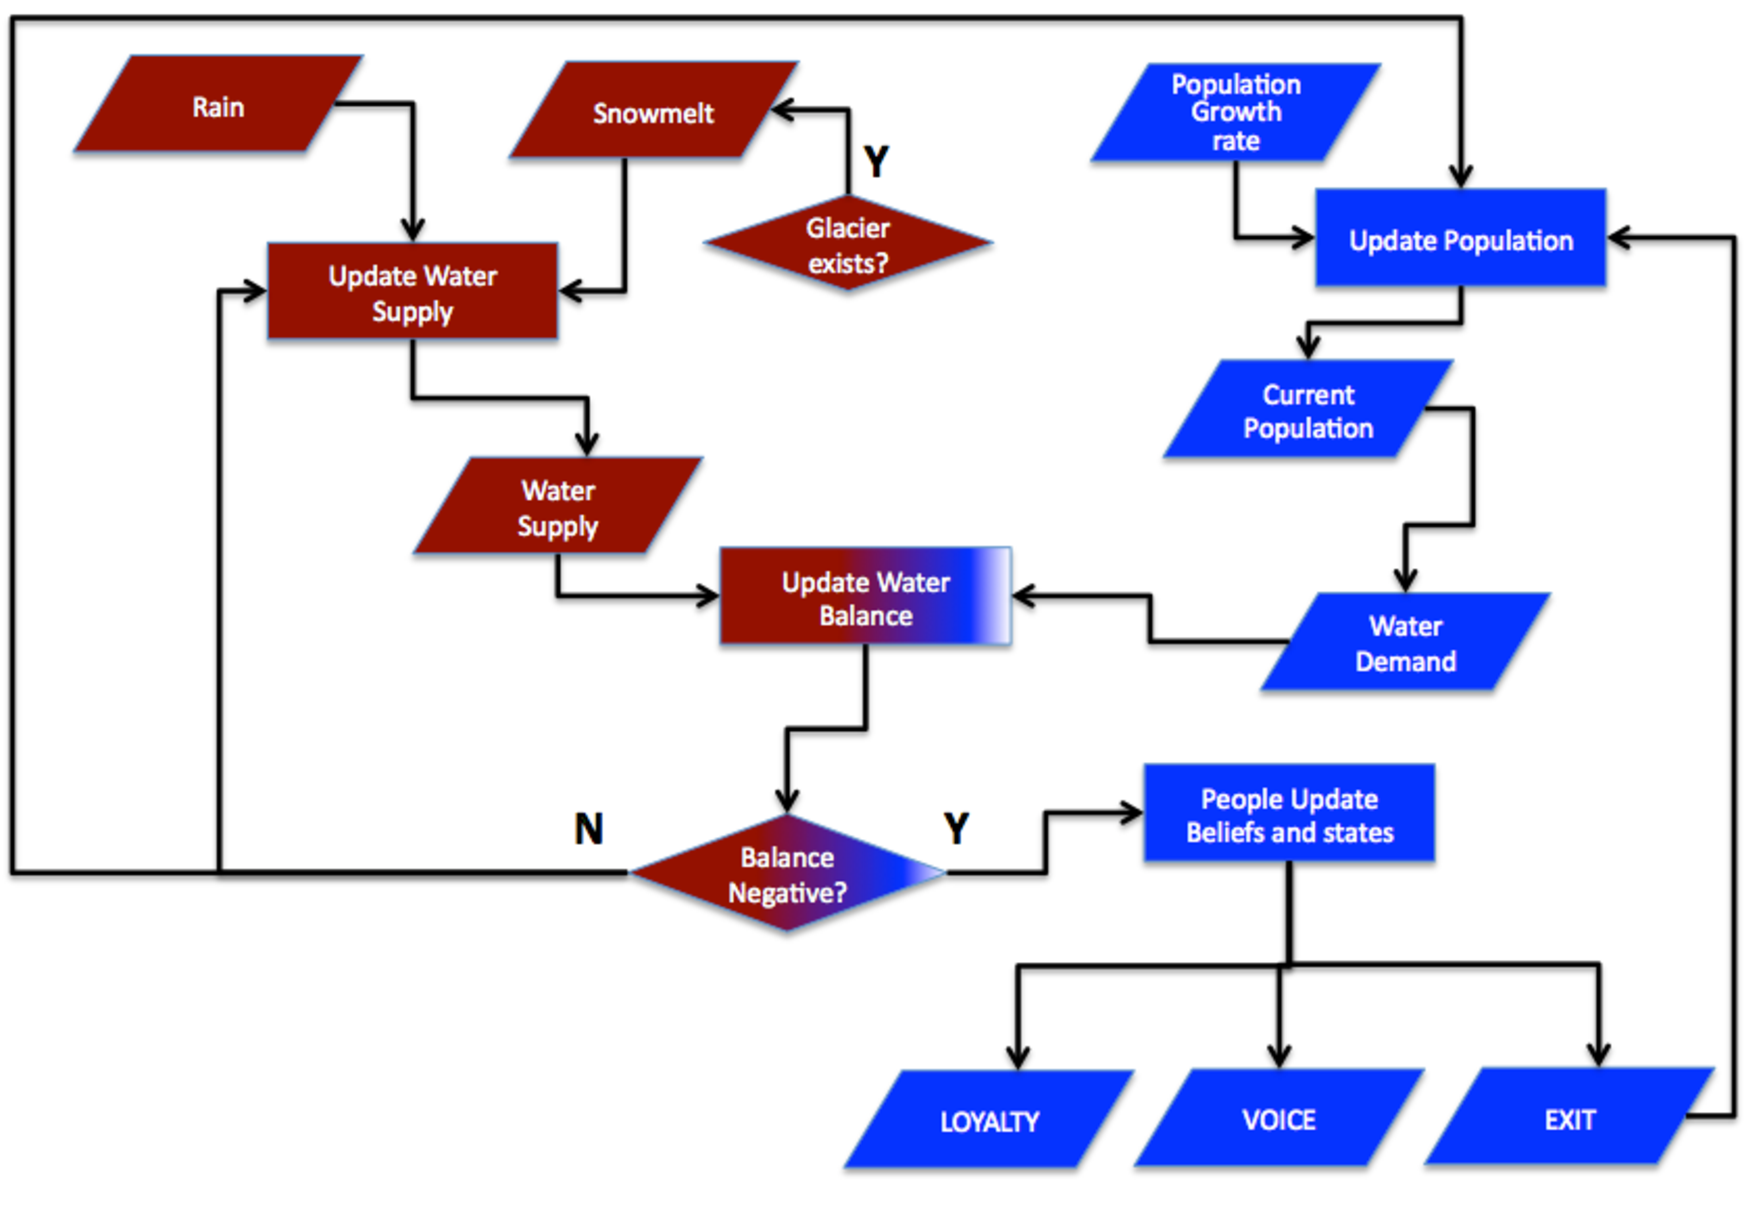
\includegraphics[width=0.7\textwidth]{flow1}
  \caption[Process Overview]{Process Overview. Color differentiates type of system (blue for  \emph{Social} and red for \emph{Natural}. A pass through this chart represents a six month \emph{season}.}
  \label{flow1}
  %%\figSpace
\end{figure}

Figure \ref{ruralLogic} is a flowchart representing the decision making of a rural agent. As it is shown in that figure, the decision flow starts when the agent detects scarcity. That detection is a particular computation following a Bayesian approach, which was the assumed as the mechanism to update beliefs. Once the agent detects scarcity, he will look for a place to move. As long as the agent detects scarcity where the agent is staying, the agent will move. The moving will end when the agent reaches the resilience limit. If the rural agent can migrate, the rural agent will migrate to the urban area. Agents that could not migrate are candidates to feel relatively deprived.

\begin{figure}[ht]
%%\figSpace
\centering
  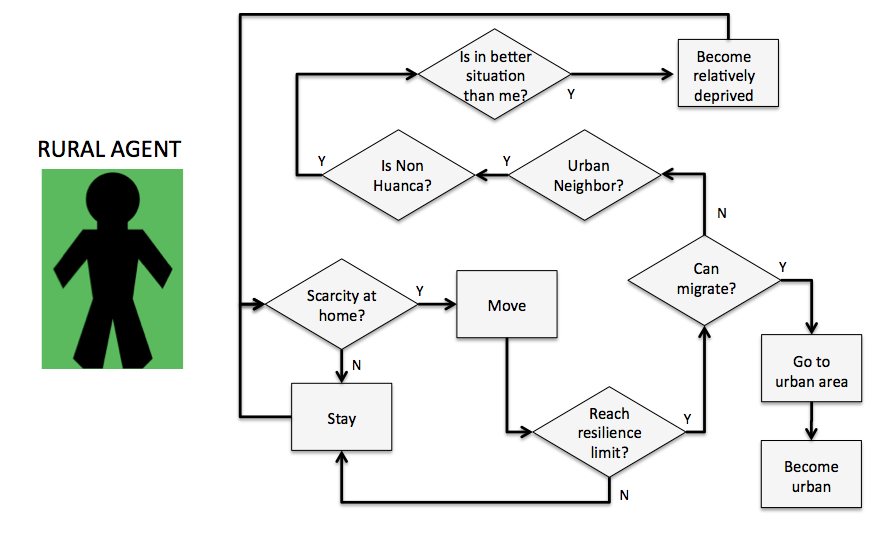
\includegraphics[width=0.7\textwidth]{ruralLogic}
  \caption[Decision making - rural agents]{Decision making - rural agents}
  \label{ruralLogic}
\end{figure}

Figure \ref{urbanLogic} is a flowchart representing the decision making of an urban agent. Similar to the previous figure, the decision flow starts when the agent detects scarcity following a Bayesian approach. Once the agent detects scarcity, he will look for a place to move. As long as the agent detects scarcity where the agent is staying, the agent will move. The moving will end when the agent reaches the resilience limit. If the urban agent can migrate, the urban agent will migrate to Lima or the Jungle, depending on the agent\textquotesingle s characteristics (employed, educated, marital status). Agents that could not migrate are candidates to feel frustrated. Once the agent is frustrated, the agent will try to connect to other agents in the same situation. These connections make a social network of frustarted or angry agents. A link is destroyed when a member of the network of frustrated agents migrates.

\begin{figure}[ht]
%%\figSpace
\centering
  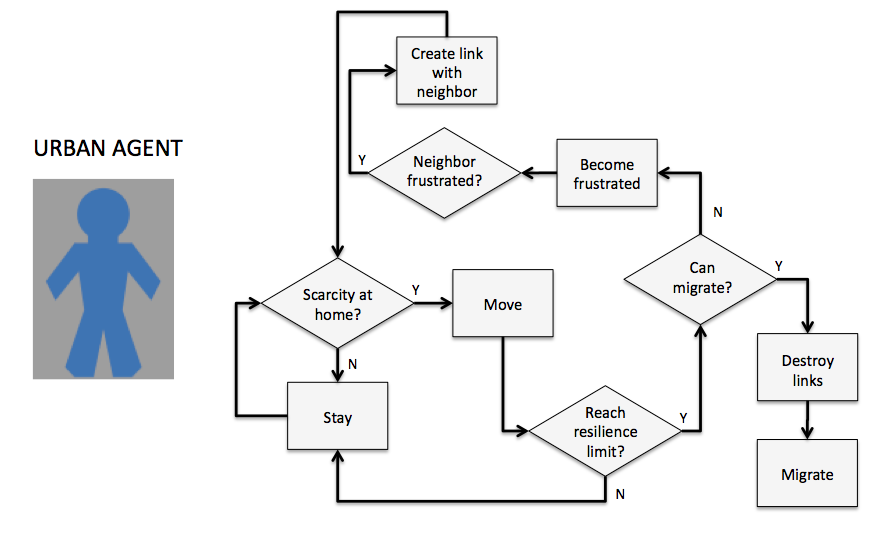
\includegraphics[width=0.7\textwidth]{urbanLogic}
  \caption[Decision making - urban agents]{Decision making - urban agents}
  \label{urbanLogic}
  %%\figSpace
\end{figure}


\section{Analysis of Results}


\begin{quote}
\emph{``Although policymakers cannot draw lessons from events that have yet to occur, they can try to anticipate events. In doing so, they may treat the future as an extension of the present in order to bound speculation by existing knowledge. Theorists can claim future success for their prescriptions on the grounds that predictions follow logically from premises, whether or not their premises are plausible. Politicians can exploit uncertainty about the future by willfully asserting faith in their proposals, which have yet to be proven wrong (pp.91)''\cite{rose_lesson-drawing_1993}}
\end{quote}

This quote from Professor Richard Rose\footnote{Director of the Center for the Study of Public Policy at the University of Strathclyde, Glasgow} has guided the purpose of our research. In his work ``\emph{Lesson-Drawing in Public Policy: A Guide to Learning Across Time and Space}'' Rose believes anticipation allows policymakers to forgo the necessary rigors of empirical evidence, as anticipation is not a scientific endeavour but in fact a \emph{political tool} that can be used when facing uncertainty and novelty. This is particularly important when questions like \emph{When will this occur?} \emph{What will be the impact?} \emph{Whom will they impact more?}  and the like, have no clear answer. These same questions are asked by policy makers and stakeholders about Huancayo, but each from his position without integrating the partial data and knowledge they have.

\begin{itemize}
\item {\bf Take one}. The model has been verified and validated. All the population is situated in the year 2011 and the model is ready to run. The population count reflects a proportion of actual population. The areas are also proportional. The Glacier Huaytapallana area in the year 2011 is represented by the zone in white, the rural settlers inhabit the green area and the urban agents are in the gray area. The water balance is not an issue yet, the water supply is enough for the population water needs. 

\begin{figure}[h]
  %\figSpace % This adds separation
  \centering
  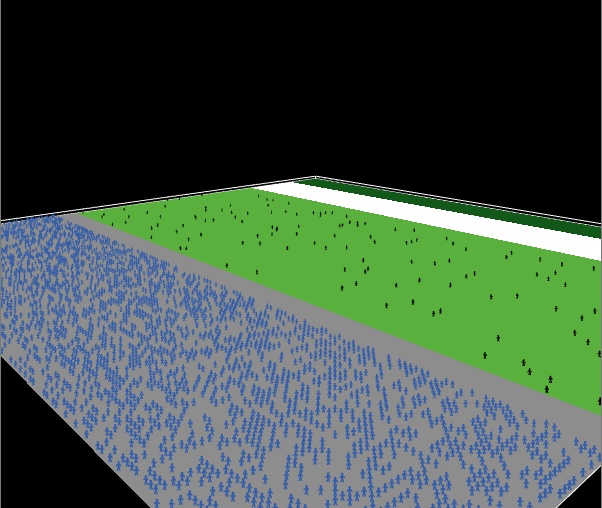
\includegraphics[width=0.6\textwidth]{esc1}
  \caption{Start of the simulation}
  \label{network}
  %%\figSpace % This adds separation
\end{figure}

\item {\bf Take two}. As time passes by, the glacier Huaytapallana keeps melting following the identified trend. The pink patches near the white patches represent the zone retreated. Even though there are no water issues in this moment, people started slowly moving away from the more densely populated area (left gray area) into the peri urban area. The only driving force for this is the population growth. 

\begin{figure}[h]
  %\figSpace % This adds separation
  \centering
  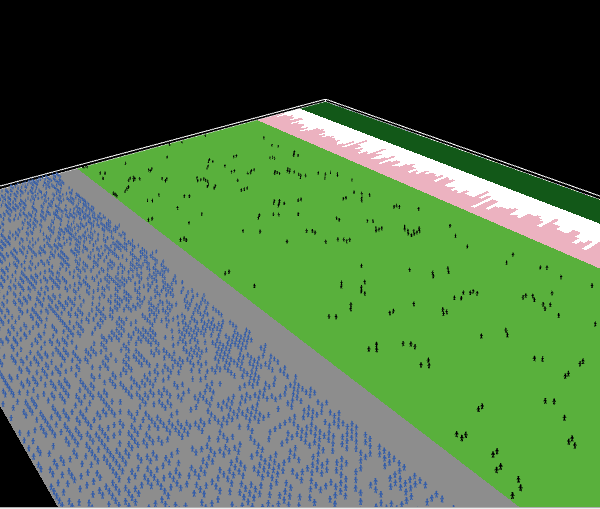
\includegraphics[width=0.6\textwidth]{esc2}
  \caption{Melting of the Huaytapallana}
  \label{network}
%  %\figSpace % This adds separation
\end{figure}

\item {\bf Take three}. The glacier has almost retreated completely and the water balance for the urban area is now negative. The pink patches in the urban area are affected by the drought during the \emph{dry season}. The drought is felt progressively from the highest risk zones (letfmost gray zone).  If an agent is living in a patch that suffers drought, he may need to move away, depending on his beliefs of future scarcity. There are some urban agents that could not migrate when their resilience was reached. They are already organizing into a network. The peri urbanization process continues but no rural is feeling relatively deprived yet.

\begin{figure}[h]
  %\figSpace % This adds separation
  \centering
  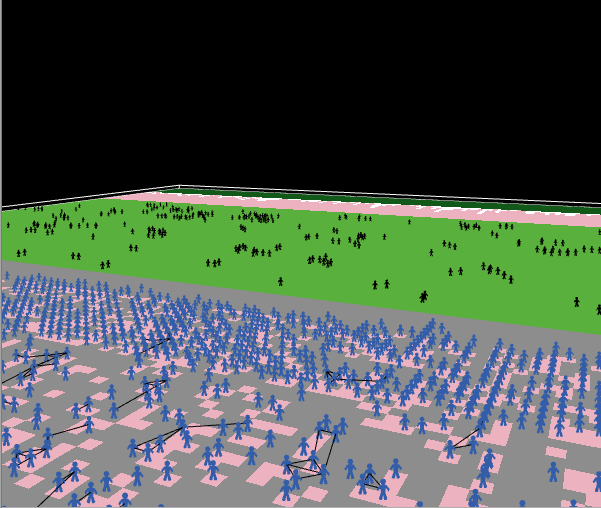
\includegraphics[width=0.6\textwidth]{esc3}
  \caption{Water scarcity and network of urban people frustrated}
  \label{network}
%  %\figSpace % This adds separation
\end{figure}

\item {\bf Take four}. The Huaytapallana has melted completely. The has made the situation even worse during the dry season. Urbans are population more the peri urban area, and the increasing presence of non Huancas has started making rural Huancas feel relatively deprived. The rural agents with a bigger size represent those rural agents. Even though the migration into Lima and the Jungle has been massive, theer are still many people feeling frustrated living in Huancayo. Not every frustrated urbanite is connected to one another, but there are many network components and cliques every where in the city. The simulation is about to finish after representing 50 years. The potential for conflict and migration turn into a fact in the model.

\begin{figure}[h]
  %\figSpace % This adds separation
  \centering
  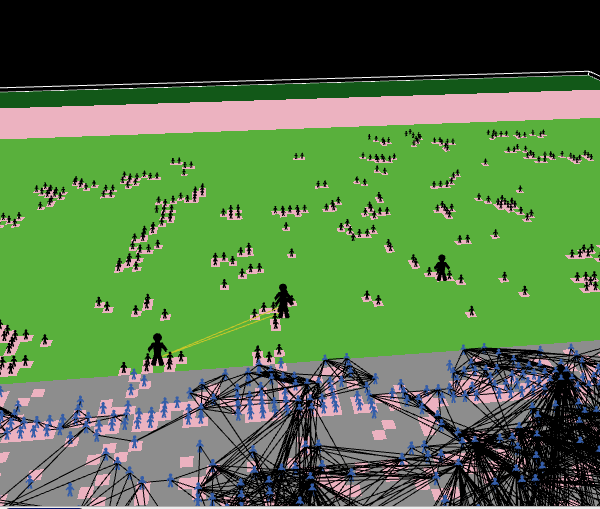
\includegraphics[width=0.6\textwidth]{esc4}
  \caption{Water scarcity, urban people frustrated and relatively deprived rural settlers}
  \label{network}
%  %\figSpace % This adds separation
\end{figure}


\end {itemize}


\clearpage

\section {Is drastic migration possible?}

Related to migration, table \ref{migra-out} informs the final values obtained. There, one can see that, even though it is possible for rurals to migrate, the balance of water in the urban area the next years would not be an issue, so even though migration is allowed for rurals in the code, no immigration took place. Migration started at period 54 (year 27) and the most dramatic migration happened in moment 64, 10 periods later (year 32). If the demographic conditions held true, the migration to the jungle would be the most alarming.

\begin{table}[ht]
  %\tableSpace % This adds separation
  \centering
  \caption{Migration-related results}
{\scriptsize
% latex table generated in R 3.0.2 by xtable 1.7-3 package
% Fri Jul 17 19:25:22 2015
\begin{tabular}{m{2.5in}p{0.5in}p{1.5in}}
  \hline
Variable & Value & Variable Name \\ 
  \hline
People that moved to the Jungle & 2662 & movedtojungle \\ 
  People that moved to Lima & 356 & movedtolima \\ 
  Rural people that moved to urban area &   0 & movedtohyo \\ 
  Moment Migration started &  54 & moment-migrate-urban \\ 
  Max amount that emigrated in a year to the Jungle & 337 & maxjungle \\ 
  Max amount that emigrated in a year to Lima &  54 & maxlima \\ 
  Max amount that emigrated in a year & 391 & maxmove \\ 
  Moment when Max amount that emigrated in a year was reached &  64 & maxtimemove \\ 
  Moment when Max amount that emigrated in a year to the Jungle was reached &  64 & maxtimejungle \\ 
  Moment when Max amount that emigrated in a year to Lima was reached &  64 & maxtimelima \\ 
   \hline
\end{tabular}}
\label{migra-out}
 % %\tableSpace % This adds separation
\end{table}


\section {Is social conflict possible?}


The Table \ref{conflict-out} informs that the simulation ended with a non Huanca population representing 72\% of the total population, that is, after 100 periods (50 years), the non Huanca population share doubled.It is also clear the share of rural people has reached 16\% (an increase of 12\%). An important value to consider is that only 3 people felt relatively-deprived, however that may include their families in case of conflict, as discussed in chapter two.

\begin{table}[ht]
  %\tableSpace % This adds separation
  \centering
  \caption{Conflict-related results}

% latex table generated in R 3.0.2 by xtable 1.7-3 package
% Fri Jul 17 19:25:27 2015
{\scriptsize
\begin{tabular}{m{3.75in}p{0.4in}p{1.3in}}
  \hline
Variable & Value & Variable Name \\ 
  \hline
Max amount of angry people reached & 2497.00 & maxmass \\ 
  Density of Angry Network when max amount of angry people reached & 0.01 & maxdensitymass \\ 
  Average clustering coefficient of Angry Network when max amount of angry people reached & 0.41 & maxmeancc \\ 
  Number of network components when Max amount of angry people reached & 491.00 & maxcomp \\ 
  Moment when Max amount of angry people reached & 96.00 & maxmassangrytime \\ 
  Rural population when max amount of angry people reached & 569.00 & maxmasspoprural \\ 
  Urban population when max amount of angry people reached & 3116.00 & maxmasspopurban \\ 
  Moment that first rural started feeling relatively deprived & 80.00 & moment-conflict-rural \\ 
   \hline
\end{tabular}
}
\label{conflict-out}
  %\tableSpace % This adds separation
\end{table}



Table \ref{conflict-out} also informs that after running the simulation for 100 periods (50 years), the possibility of conflict in the rural area started around the period 80 (year 40). On the other hand, in the urban area the network of angry people does not get to reach high values, which means that though there are many angry people, very few of them are connected. However, that result should need further reflection. These results could get the reader wrong if no other measure of connectivity had been obtained. Fortunately, we are aware that the low density does not mean a low potential for conflict, but that there are many components, some of them very tightly connected that could make and escalate conflict. A sample network in a moment of maximum angry people is shown in Figure \ref{network}, showing how unmanageable this situation could become.

\begin{figure}[h]

  \centering
  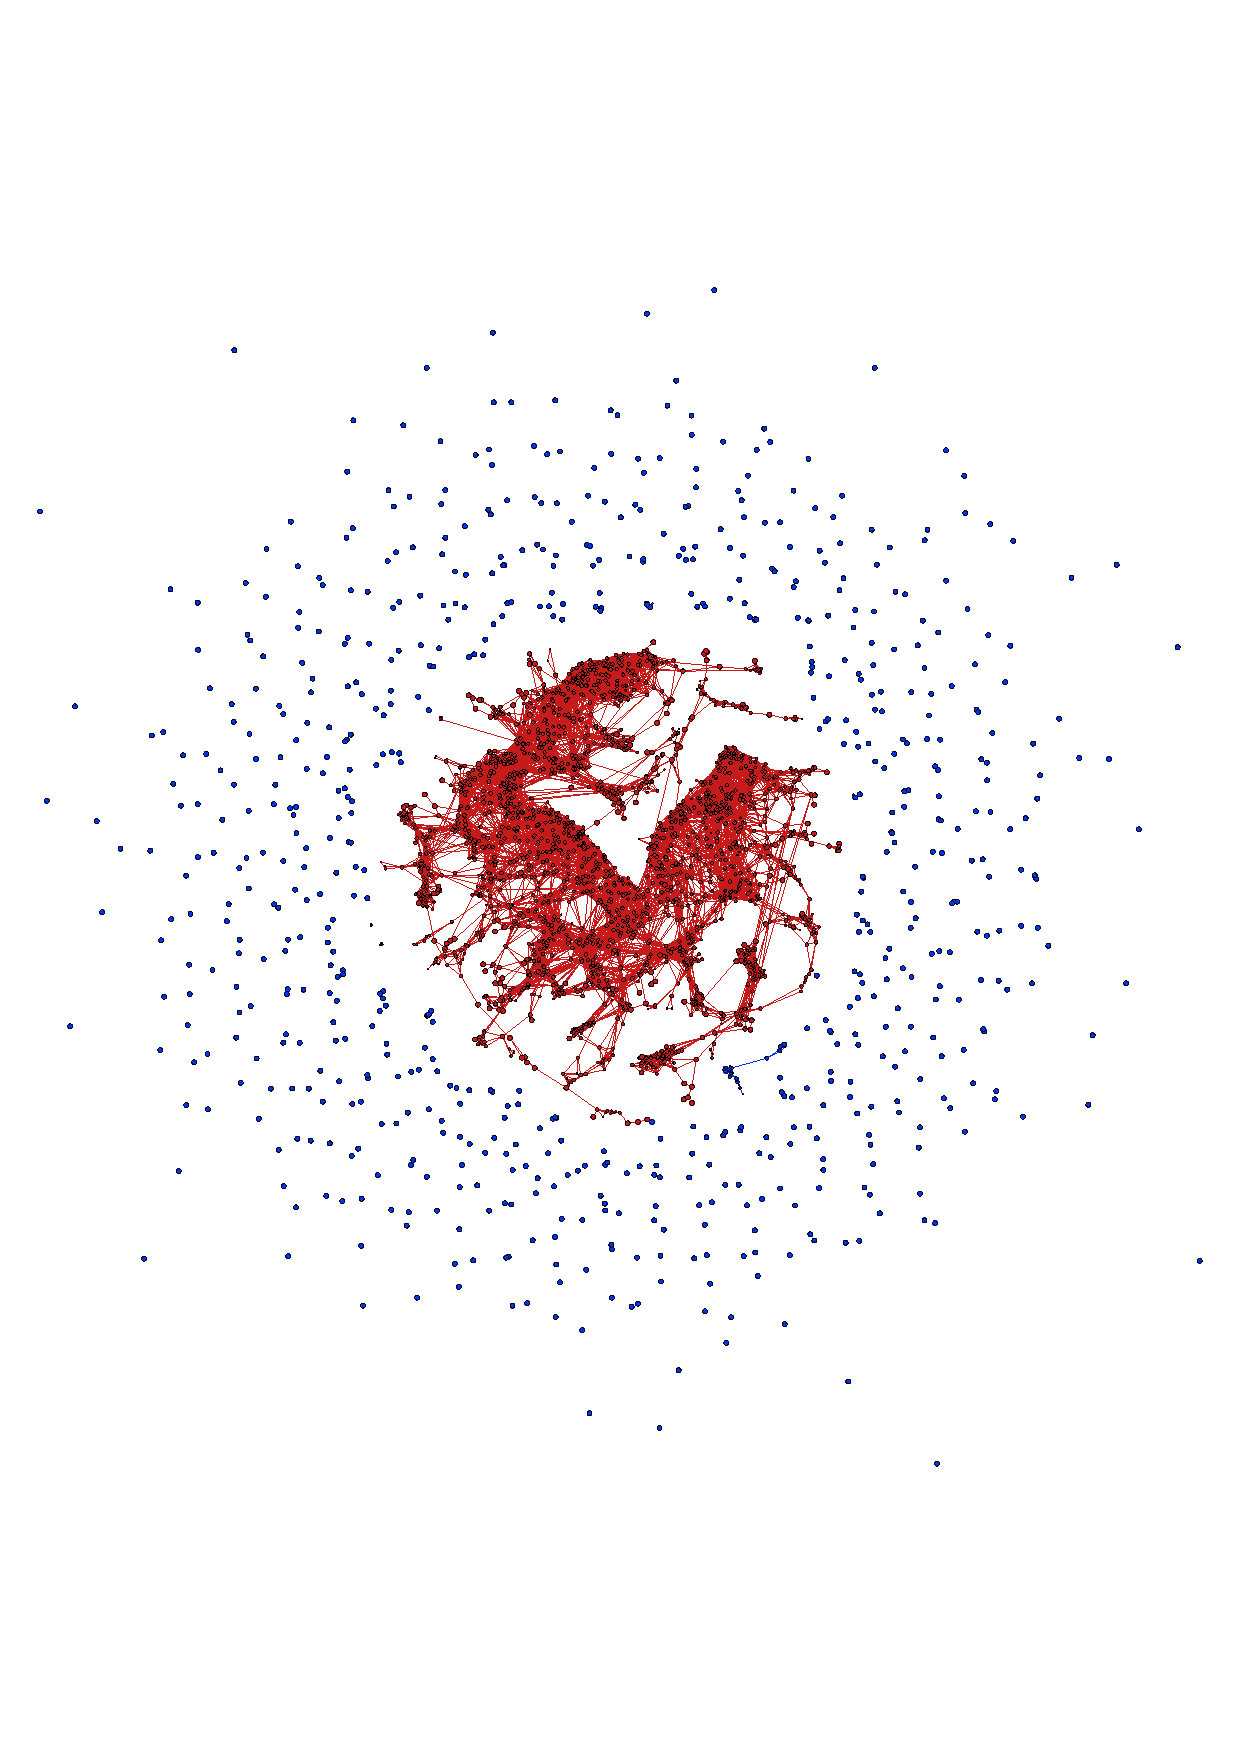
\includegraphics[trim = 0cm 5cm 0cm 5cm,clip,width=0.75\textwidth]{network}
  \caption[Network of Angry People]{Network of Angry People. This is a network during the moment when the maximum amount of angry people was reached. You can see isolates and  components. This network has an average clustering coefficient= 0.3635, 705 connected components and a density = 0.007}
  \label{network}
  %\figSpace % This adds separation
\end{figure}



\section{Discussion and Conclusions}

The natural barrier to anticipation is a reactive mindset, which is very common in policy making \cite{torjman_what_2005}. For sure, one can not blame decision makers for being reactive as generally the political institutions are a set of rules that have been conceived based on what is known. There may be many examples of catastrophes that could have been avoided if the right anticipatory measure had been taken previously, but it is also true that the legal systems generally lack means to make decision makers liable for their lack of planing; and  only electoral means are a way to express the general discontent for their lack of proactiveness. However, electing a new or better political leader does not undo the damage and suffering of the affected people. A reactive system of policies is not completely bad, and could even be considered an efficient way of spending public moneys. However, when combined with other factors, the whole situation can become catastrophic. 

A first negative ingredient can be extremely centralized systems or weakly decentralized. A centralized system will react only after every institution beneath has considered that there is a need for anticipation, and a weekly centralized system gives the local institutions the illusion of decision making, when in reality there is a regulation that will force the local authority to deal with a complicated set of institutions. The Shullcas and the Huaytapallana are clearly affected by this situation. Another negative ingredient to reactive policy-making is symbolic and superficial proactiveness. Particularly when dealing with this climate change issue, programs and organizations are created, technical documents are produced, presentations and dinners are offered, but at the end there is clear taste of no real measures. 

The level of economic development is also a key factor in understanding the ability to cope with water shortages, as more developed countries have more technological and financial resources to deal with drastic environment issues, while poorer regions, countries, or localities have meager funds and often suffer through political instability that constrains implementation of effective and long-lasting policies. However, economic development has not stopped advance economies like the USA to be reactive in many cases in many different issues like the Challenger accident, the 9/11, Katrina hurricane, and so on (for more stories see \cite{bazerman_predictable_2004}). Then, poor leadership affects enormously a reactive system of policies. A poor leader plays safe, and tends to leave difficult situations to \emph{experts}, framing complex issues as \emph{technical}.  As explained by Heifetz and Linsky \cite{heifetz_leadership_2002}, 
once leaders frame a complex problem as technical instead of complex-adaptive the political system just does ``routine management'' instead of ``change management''. This explains that the reports on the watershed appeared around 2010, and all of them were very technical; and since then, no more knowledge on this area has been produced from the government.



\section{Beyond the model}

{\bf What should be improved in the model?} \\
Every model needs assumptions and facts, those facts can be qualitative or quantitative, and this agent based model has dealt very well with facts and assumptions. However, the most urgent areas of improvement can be:
\begin{itemize}
\item Have a better sub model of what an agent could do when it predicts water scarcity is important. In our model, the agent looks for another sources of water, and when the agent finds a better place it abandons its home and moves to another place within the system, and keep doing that until his desire to stay in the system is surpassed. However, we would have preferred to have information on neighborhoods and its economic capacity, to implement an algorithm considering that information, but that data does not exist. An important investment would be needed to produce that data.
\item This model assumes to main destinations for the emigrants from Huancayo, Lima and the Jungle, but Lima in fact represents ``big cities in the coast'' and the Jungle represent ``good places to go if you are a risk taker and your are not planing to bring your family''; although the answers from the interviews mentioned these two places it would be important to expand the model and see how the new arrivals are received and what new issues arise in those destinations. The answers also mentioned ``foreign countries'', but that destination has not been included (but ``Lima'' could represent it).
\item It would be important to consider more strategies of the agent according to its economic capacity. The economic capacity is unknown at agent level, so further work on this should be done. It is important also to conduct a more detailed analysis on water regulation from the government to get the agents reduce consumption; since Peru is a country where no political authority wants to alter the price of water (water is very cheap in Peru), a different regulation mechanism should be thought following a participatory approach.

\item A different programming platform could be important to consider. At this point, we have reached the capacity of NetLogo but if this model becomes more computing-intensive, there is clear need to migrate the model into Mason, Repast or Gamma. In fact, the code is ready to be sent to real maps, and see the simulation in a more realistic setting, but those other ABM platforms are needed to make the conversion useful. 
\end{itemize}


{\bf What measures should be taken?}

This model, despite the real data that has been used to feed it, is still more a political tool than a engineering one. Its purpose is to show potential and not clear forecast of counts and moments, but a clear picture of what might happen and what to do to avoid it or gain time. This model\textquotesingle s ultimate goal is to raise enough awareness that triggers real political action. With that in mind, there are some recommendation on the next steps policy makers should follow:

\begin{itemize}
\item \emph{Make sure people in rural area have enough rights and mechanisms to stay in their lands in good conditions.} The tendency of immigration may not diminish in the short run and rural people have no intention to leave Huancayo. To avoid relative deprivation emerge, policy makers from the central government need to assist rural populations to adapt their farming practices; regional planers need to determine buffers that separate urban from rural area as well as assure minimal literacy conditions; while local governments need to stop giving building permits in the buffer area. The local University may also contribute to raise competitiveness of the local production.

\item \emph{Create mechanisms to ensure political participation of rural people.} Rural people are politically under represented. They only have local committees that regulate their internal activities in the community; but they have no real presence in the regional decision making. Local and regional governments should make sure that rural people have voice in every meeting held monthly where their participation will avoid future discrepancies. Policy makers have to keep in mind that the model is constantly recommending to increase the water reserve from the rainy season, which will need investment and the use of arable and/or herding land; in either case, rural communities will feel they are affected to favor exclusively the urban.

\item \emph{Improve participatory water governance.} The distribution of water between rural and urban area is currently a process that represents a constant debate. From the interviews, rural people believe that the city is taking more than water than they should from the Shullcas during the dry season and that the rural needs are relegated due to the pressure of the urban majority. Water management has many actors involved, including two Ministries from the central government (Agriculture and Environment), but the technical criteria adopted so far is biased toward the needs of the urban area. 


\item \emph{Create and save the institutional memory.}This model has been done in the USA, but very distant from the modeling conditions we are familiar. Developed countries have long understand the importance of collecting, organizing and sharing data for the research community to find research problems and propose different solutions, or more importantly, to keep a memory of the events a community has experienced and help their local analysts do their job. Peru is the opposite. 

\item \emph{Do not hide the crisis, but show a plan.} The dramatic situation has to be shared with the population, but in a message that shows the local governments have a plan that needs urban people to alter their inefficient use of water, or to learn routines that avoid unnecessary use of water. If the water demand decreases in the long run, make sure this process gets as slow as possible. For that, different campaigns should be promoted at elementary and high school level to be more efficient using water in the future generations of \emph{Huancainos}; organize contests at college level to promote local inventions; and organize neighborhood contests to demonstrate how to achieve efficient practices in the use of water.

\item \emph{Seek collaboration from civil society, especially research institutions.} The highlands of Peru have been always scenarios for NGOs to operate. Ideally, NGOs detect social problems and work with the community to empower their actors; but this time the challenge is different, as it deals with the resilience and adaptive capacity of people facing high uncertainty of the future environmental conditions and the reactions their neighbors themselves will have in those critical moments. In this situation, the production of more knowledge is needed as well as interdisciplinary debate. The government has serious limitations to hire people permanently, but the local public University is the forgotten partner that could make all the difference. The local University has enough resources to fund important programs that can keep updating the social and natural situation for more informed policy making and modeling, and which should create mechanisms for a two-way knowledge transfer, that is share scientific knowledge and collect traditional knowledge. 
\item \emph{Be careful of easy solutions.} This work has suggested many times the saving of water. This is a decision that needs to be very well planned. To start, a huge reservoir for the area seems to be a good solution, but decision makers have to be aware of the Huaytapallana failure. This failure can cuase any time a huge earthquake, and a huge reservoir represents a great potential for disaster. The saving of water will need a lot of work from the political class and the people themselves. From the top down, the infraestructure to save or become more efficient shpuld be built; and the urban and rural settlers have the responsibility to be more efficient using water. Another important way to secure water will be a better management of the ground water, which currently is used without detailed knowledge of its quantitity nor quality, and without any recharging policy.

\end{itemize}





\printbibliography

\end{document}

